\chapter{ANALISIS DAN PERANCANGAN}

\section{Analisis Masalah}

Hampir semua studi pengembangan algoritma estimasi \textit{world model} yang melacak posisi robot maupun bola di kontes robot sepak bola mengasumsikan bahwa komunikasi antar robot memiliki latensi yang dapat diabaikan dan belum ada yang mencoba menangani secara eksplisit dan menganalisis pengintegrasian data dari robot lain yang terlambat. Secara umum, masih sedikit studi yang membahas penggabungan data pengukuran sensor dengan latensi pada sistem komputasi terdesentralisasi.

\section{Lingkungan Implementasi}

\begin{figure}[h]
    \centering
    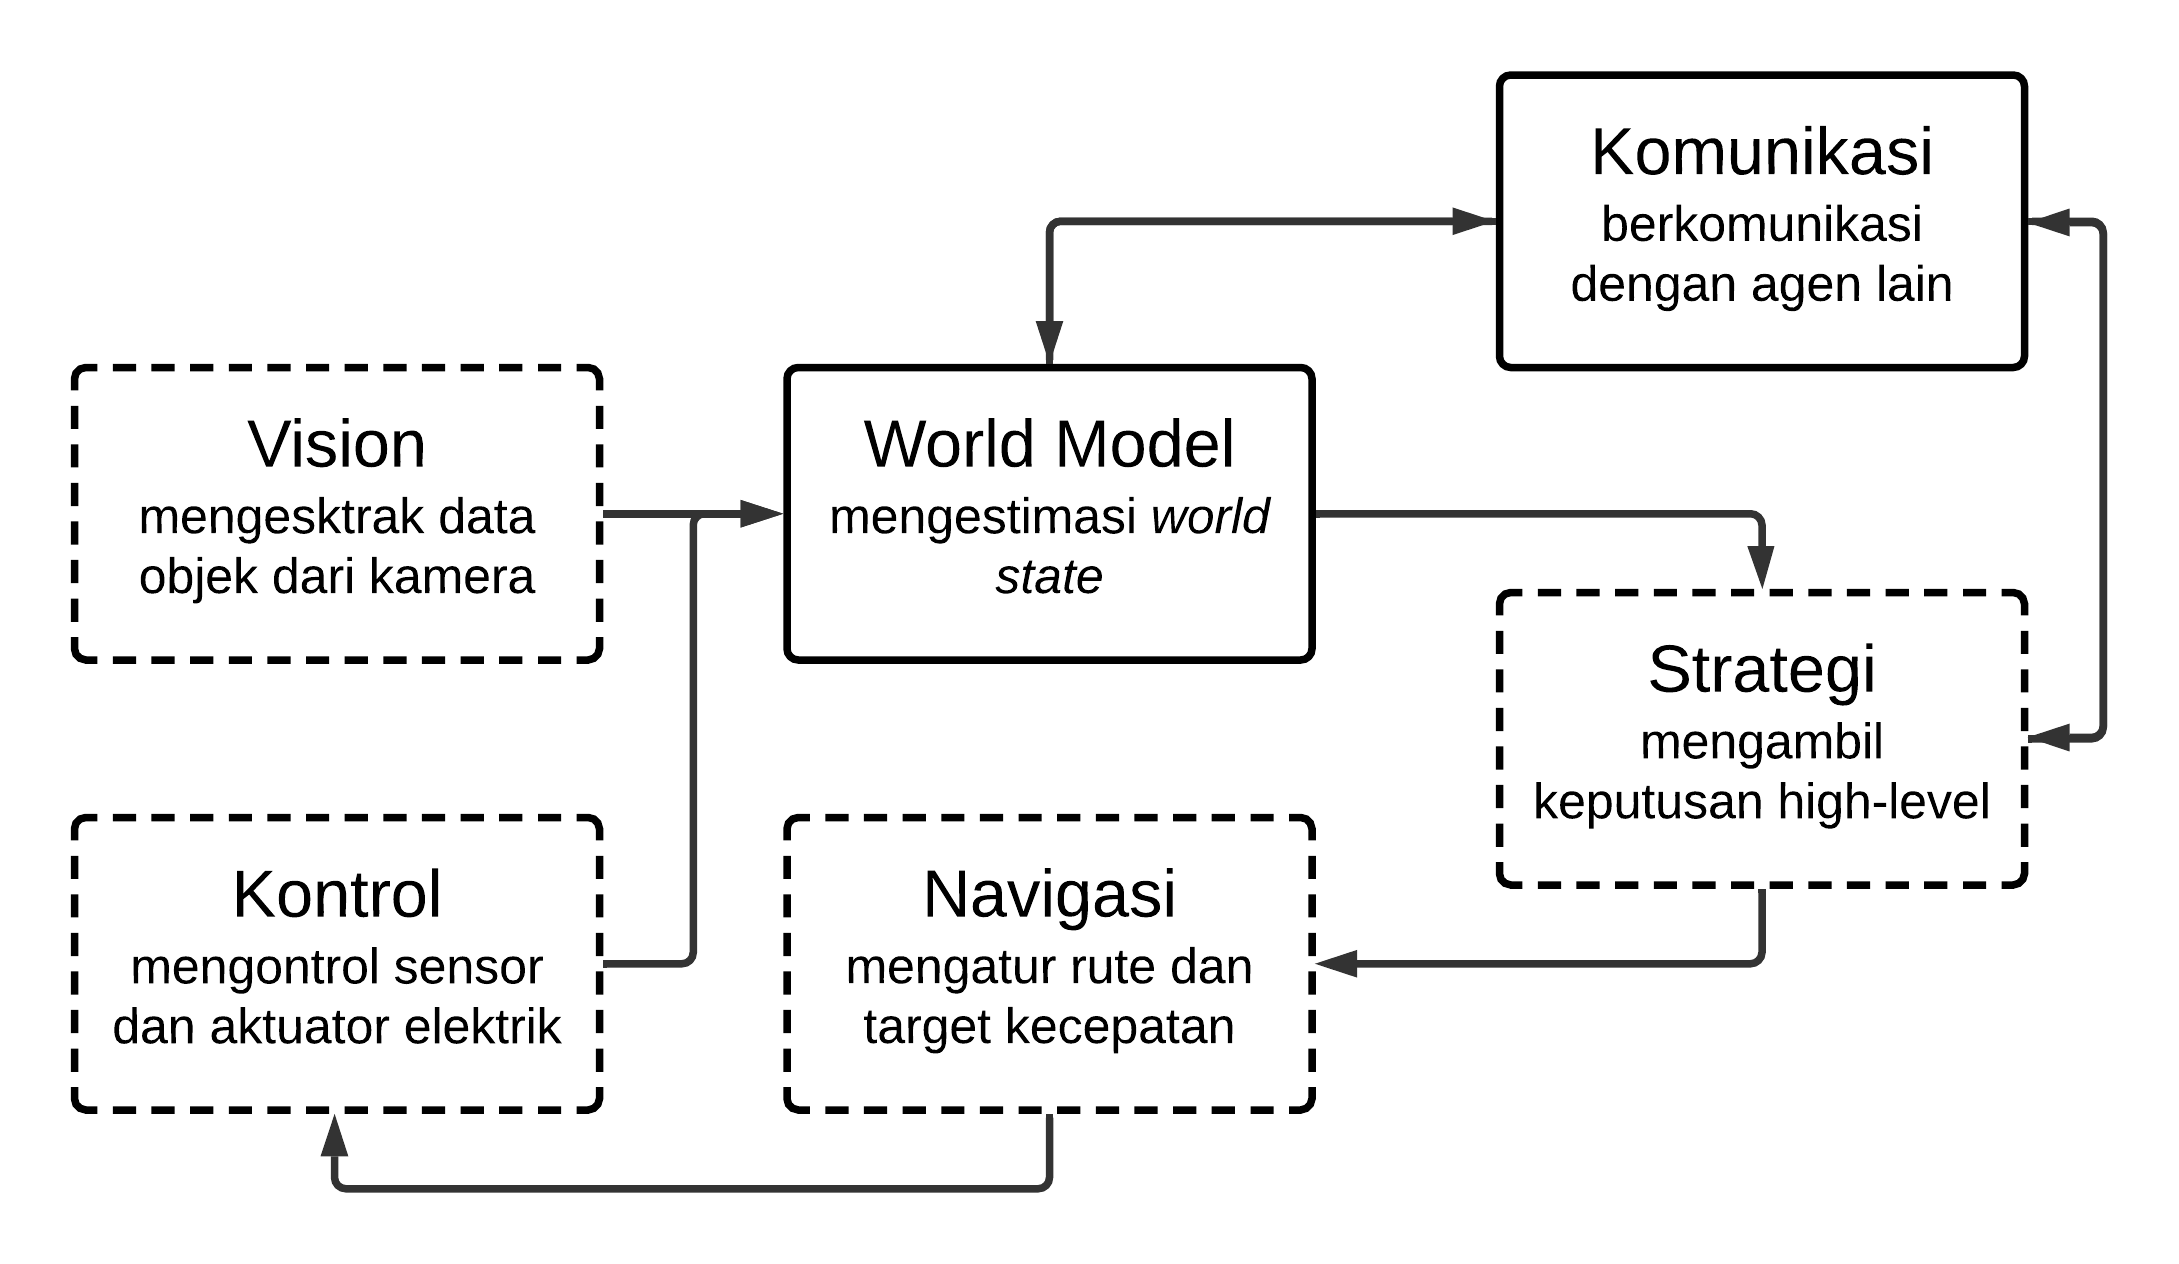
\includegraphics[width=0.8\textwidth]{resources/dagozilla-structure.png}
    \caption{Struktur modul Dagozilla}
    \label{fig:dagozilla-structure}
\end{figure}

Lingkungan perangkat lunak DAGOZILLA menggunakan \textit{platform} \textit{Robot Operating System} (\textit{ROS}) yang memungkinkan komunikasi antar proses oleh modul-modul aplikasi yang menjalankan fungsi-fungsi robot menggunakan paradigma \textit{publish-subscribe} pesan atau \textit{request-response} \textit{service} yang disediakan suatu modul. Modul-modul yang ada digambarkan pada gambar \ref{fig:dagozilla-structure}.

Fokus utama dari tugas akhir ini adalah mengembangkan modul \textit{world model} yang bertugas untuk memproses semua data persepsi dari modul sebelumnya maupun informasi dari robot lain untuk menyediakan estimasi keadaan dunia yang seakurat dan sefaktual mungkin agar dapat digunakan dalam melakukan pengambilan keputusan.

Modul kontrol berkomunikasi dengan mikrokontroler yang berhubungan langsung dengan \textit{hardware} untuk mengontrol aktuator dan mengambil data dari sensor-sensor lokal, diantaranya odometri motor penggerak dan kompas. Odometri mengukur perputaran yang dilakukan masing-masing roda penggerak yang dapat diolah menjadi data perpindahan dan kompas mengukur orientasi global dari robot itu sendiri.

Modul \textit{vision} mengekstrak data dari kamera, diantaranya posisi bola dari gambar menggunakan deteksi warna dan momen objek, dan sebaran titik dari garis lapangan maupun objek penghalang lapangan menggunakan algoritma \textit{radial search line}.

\section{Analisis dan Desain Umum Solusi}

Sebagai gambaran besar hipotesis solusi, masing-masing robot tetap harus melakukan estimasi sendiri menggunakan data yang tersedia dari sensor lokal robot tersebut. Hal ini dilakukan agar masing-masing robot harus tetap memiliki estimasi informasi krusial seperti posisi robot sendiri, bola, ataupun penghalang walaupun terjadi kegagalan jaringan komunikasi. Algoritma secara umum harus berjalan secara \textit{online} tanpa masing-masing robot harus menunggu informasi dari robot lain terlebih dahulu sebelum dapat dijalankan. Penapis partikel dianggap sebagai metode yang cukup baik untuk melacak posisi robot maupun bola yang dapat bergerak secara bebas.

Masing-masing robot lalu menyebarkan hasil pemrosesan lokalnya ke semua robot lain. Mengirimkan keseluruhan informasi pengukuran secara mentah dianggap kurang dapat diandalkan dan meningkatkan beban komputasi untuk semua robot melihat ada data seperti persepsi garis lapangan dan objek penghalang yang terdiri dari puluhan sampai ratusan data titik. Data seperti sebaran partikel estimasi haruslah diproses dahulu ke bentuk lain seperti \textit{Gaussian Mixture Model} sebelum disiarkan ke robot lain.

Data hasil pemrosesan mengandung \textit{time-stamp} agar robot yang menerima dapat mendeteksi dan melakukan pengolahan tambahan untuk data yang terlambat. Data juga mengandung ukuran tingkat kepercayaan keakuratan yang ditetapkan robot penyiar. Hal ini dilakukan karena walaupun pertukaran informasi dapat meningkatkan akurasi, hal tersebut juga dapat menyebabkan penyebaran \textit{error} dalam estimasi, sehingga harus didesain sehingga informasi dengan tingkat kepercayaan yang rendah tidak terlalu mempengaruhi informasi dengan tingkat kepercayaan yang lebih tinggi.

Diagram alir hipotesis solusi digambarkan di \ref{fig:solution-flowchart}.

\begin{figure}[h]
    \centering
    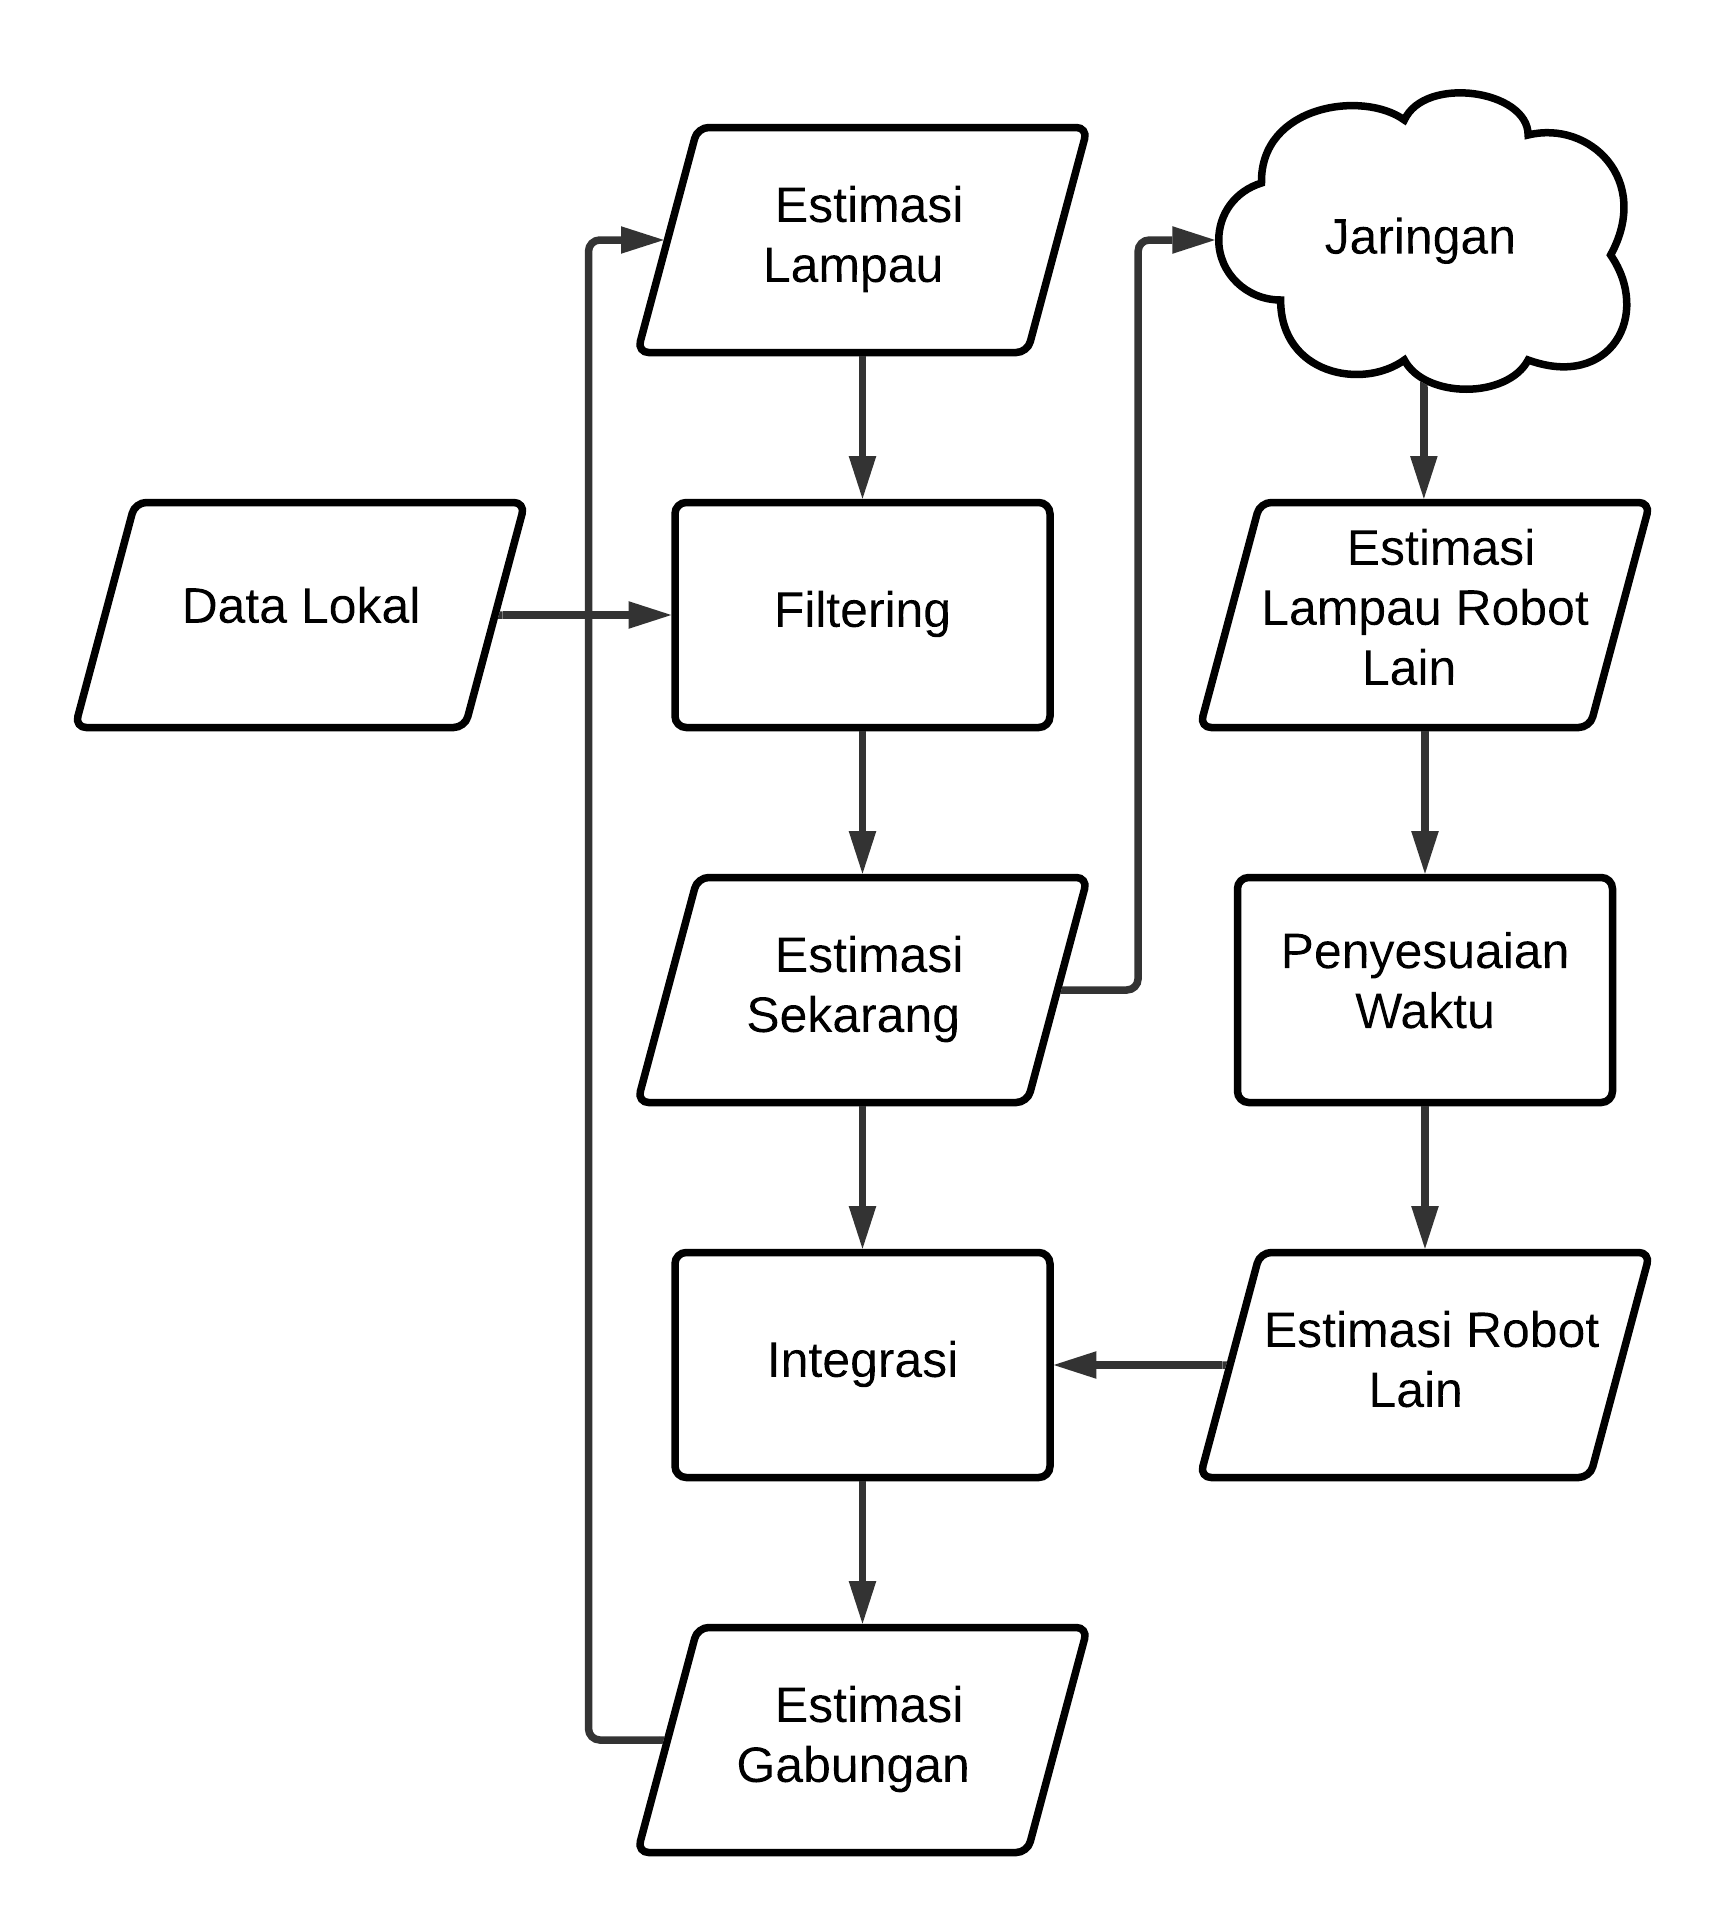
\includegraphics[width=0.8\textwidth]{resources/solution-flowchart.png}
    \caption{Diagram alir hipotesis solusi}
    \label{fig:solution-flowchart}
\end{figure}